% Created by tikzDevice version 0.10.1 on 2018-03-04 15:38:57
% !TEX encoding = UTF-8 Unicode
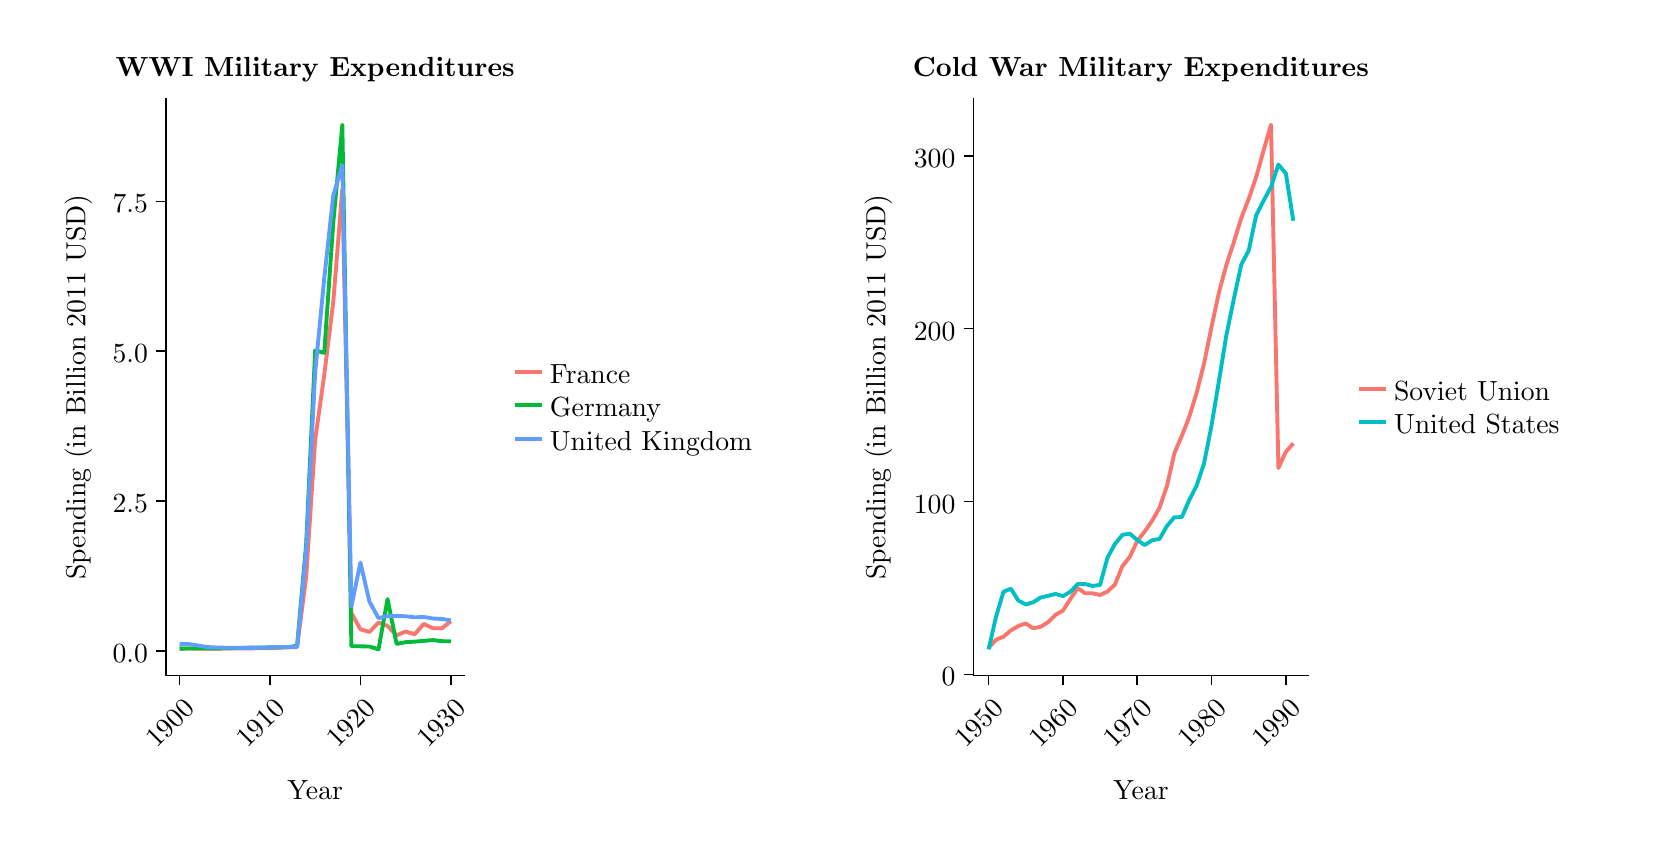
\begin{tikzpicture}[x=1pt,y=1pt]
\definecolor{fillColor}{RGB}{255,255,255}
\path[use as bounding box,fill=fillColor,fill opacity=0.00] (0,0) rectangle (578.16,289.08);
\begin{scope}
\path[clip] ( 49.97, 54.95) rectangle (157.82,263.47);
\definecolor{drawColor}{RGB}{248,118,109}

\path[draw=drawColor,line width= 1.4pt,line join=round] ( 54.87, 64.71) --
	( 58.14, 64.74) --
	( 61.41, 64.70) --
	( 64.68, 64.68) --
	( 67.94, 64.67) --
	( 71.21, 64.74) --
	( 74.48, 64.82) --
	( 77.75, 64.78) --
	( 81.02, 64.80) --
	( 84.29, 64.85) --
	( 87.55, 64.90) --
	( 90.82, 65.03) --
	( 94.09, 65.16) --
	( 97.36, 65.27) --
	(100.63, 90.58) --
	(103.89,140.19) --
	(107.16,163.56) --
	(110.43,190.01) --
	(113.70,230.80) --
	(116.97, 77.58) --
	(120.24, 71.67) --
	(123.50, 70.73) --
	(126.77, 74.14) --
	(130.04, 72.89) --
	(133.31, 69.50) --
	(136.58, 70.86) --
	(139.85, 69.92) --
	(143.11, 73.62) --
	(146.38, 72.09) --
	(149.65, 72.02) --
	(152.92, 74.63);
\definecolor{drawColor}{RGB}{0,186,56}

\path[draw=drawColor,line width= 1.4pt,line join=round] ( 54.87, 64.69) --
	( 58.14, 64.74) --
	( 61.41, 64.75) --
	( 64.68, 64.74) --
	( 67.94, 64.75) --
	( 71.21, 64.83) --
	( 74.48, 64.88) --
	( 77.75, 64.95) --
	( 81.02, 65.08) --
	( 84.29, 65.10) --
	( 87.55, 65.14) --
	( 90.82, 65.16) --
	( 94.09, 65.21) --
	( 97.36, 65.74) --
	(100.63,102.49) --
	(103.89,172.44) --
	(107.16,171.57) --
	(110.43,218.71) --
	(113.70,254.00) --
	(116.97, 65.56) --
	(120.24, 65.54) --
	(123.50, 65.45) --
	(126.77, 64.43) --
	(130.04, 82.59) --
	(133.31, 66.40) --
	(136.58, 67.03) --
	(139.85, 67.22) --
	(143.11, 67.49) --
	(146.38, 67.79) --
	(149.65, 67.39) --
	(152.92, 67.35);
\definecolor{drawColor}{RGB}{97,156,255}

\path[draw=drawColor,line width= 1.4pt,line join=round] ( 54.87, 66.42) --
	( 58.14, 66.36) --
	( 61.41, 65.85) --
	( 64.68, 65.27) --
	( 67.94, 65.12) --
	( 71.21, 65.03) --
	( 74.48, 65.00) --
	( 77.75, 64.98) --
	( 81.02, 64.95) --
	( 84.29, 65.05) --
	( 87.55, 65.16) --
	( 90.82, 65.24) --
	( 94.09, 65.30) --
	( 97.36, 65.29) --
	(100.63,100.19) --
	(103.89,164.59) --
	(107.16,198.42) --
	(110.43,228.47) --
	(113.70,239.38) --
	(116.97, 79.97) --
	(120.24, 95.79) --
	(123.50, 81.69) --
	(126.77, 75.72) --
	(130.04, 76.48) --
	(133.31, 76.48) --
	(136.58, 76.40) --
	(139.85, 76.02) --
	(143.11, 76.13) --
	(146.38, 75.59) --
	(149.65, 75.41) --
	(152.92, 74.92);
\end{scope}
\begin{scope}
\path[clip] (  0.00,  0.00) rectangle (578.16,289.08);
\definecolor{drawColor}{RGB}{0,0,0}

\path[draw=drawColor,line width= 0.6pt,line join=round,line cap=rect] ( 49.97, 54.95) --
	( 49.97,263.47);
\end{scope}
\begin{scope}
\path[clip] (  0.00,  0.00) rectangle (578.16,289.08);
\definecolor{drawColor}{RGB}{0,0,0}

\node[text=drawColor,anchor=base east,inner sep=0pt, outer sep=0pt, scale=  1.0000] at ( 43.47, 59.70) {0.0};

\node[text=drawColor,anchor=base east,inner sep=0pt, outer sep=0pt, scale=  1.0000] at ( 43.47,113.85) {2.5};

\node[text=drawColor,anchor=base east,inner sep=0pt, outer sep=0pt, scale=  1.0000] at ( 43.47,168.00) {5.0};

\node[text=drawColor,anchor=base east,inner sep=0pt, outer sep=0pt, scale=  1.0000] at ( 43.47,222.16) {7.5};
\end{scope}
\begin{scope}
\path[clip] (  0.00,  0.00) rectangle (578.16,289.08);
\definecolor{drawColor}{RGB}{0,0,0}

\path[draw=drawColor,line width= 0.6pt,line join=round] ( 46.47, 63.83) --
	( 49.97, 63.83);

\path[draw=drawColor,line width= 0.6pt,line join=round] ( 46.47,117.98) --
	( 49.97,117.98);

\path[draw=drawColor,line width= 0.6pt,line join=round] ( 46.47,172.14) --
	( 49.97,172.14);

\path[draw=drawColor,line width= 0.6pt,line join=round] ( 46.47,226.29) --
	( 49.97,226.29);
\end{scope}
\begin{scope}
\path[clip] (  0.00,  0.00) rectangle (578.16,289.08);
\definecolor{drawColor}{RGB}{0,0,0}

\path[draw=drawColor,line width= 0.6pt,line join=round,line cap=rect] ( 49.97, 54.95) --
	(157.82, 54.95);
\end{scope}
\begin{scope}
\path[clip] (  0.00,  0.00) rectangle (578.16,289.08);
\definecolor{drawColor}{RGB}{0,0,0}

\path[draw=drawColor,line width= 0.6pt,line join=round] ( 54.87, 51.45) --
	( 54.87, 54.95);

\path[draw=drawColor,line width= 0.6pt,line join=round] ( 87.55, 51.45) --
	( 87.55, 54.95);

\path[draw=drawColor,line width= 0.6pt,line join=round] (120.24, 51.45) --
	(120.24, 54.95);

\path[draw=drawColor,line width= 0.6pt,line join=round] (152.92, 51.45) --
	(152.92, 54.95);
\end{scope}
\begin{scope}
\path[clip] (  0.00,  0.00) rectangle (578.16,289.08);
\definecolor{drawColor}{RGB}{0,0,0}

\node[text=drawColor,rotate= 45.00,anchor=base east,inner sep=0pt, outer sep=0pt, scale=  1.0000] at ( 60.72, 42.61) {1900};

\node[text=drawColor,rotate= 45.00,anchor=base east,inner sep=0pt, outer sep=0pt, scale=  1.0000] at ( 93.40, 42.61) {1910};

\node[text=drawColor,rotate= 45.00,anchor=base east,inner sep=0pt, outer sep=0pt, scale=  1.0000] at (126.08, 42.61) {1920};

\node[text=drawColor,rotate= 45.00,anchor=base east,inner sep=0pt, outer sep=0pt, scale=  1.0000] at (158.76, 42.61) {1930};
\end{scope}
\begin{scope}
\path[clip] (  0.00,  0.00) rectangle (578.16,289.08);
\definecolor{drawColor}{RGB}{0,0,0}

\node[text=drawColor,anchor=base,inner sep=0pt, outer sep=0pt, scale=  1.0000000] at (103.89, 10.00) {Year};
\end{scope}
\begin{scope}
\path[clip] (  0.00,  0.00) rectangle (578.16,289.08);
\definecolor{drawColor}{RGB}{0,0,0}

\node[text=drawColor,rotate= 90.00,anchor=base,inner sep=0pt, outer sep=0pt, scale=  1.0000000] at ( 20.89,159.21) {Spending (in Billion 2011 USD)};
\end{scope}
\begin{scope}
\path[clip] (  0.00,  0.00) rectangle (578.16,289.08);
\definecolor{drawColor}{RGB}{248,118,109}

\path[draw=drawColor,line width= 1.4pt,line join=round] (176.10,164.63) -- (185.73,164.63);
\end{scope}
\begin{scope}
\path[clip] (  0.00,  0.00) rectangle (578.16,289.08);
\definecolor{drawColor}{RGB}{0,186,56}

\path[draw=drawColor,line width= 1.4pt,line join=round] (176.10,152.58) -- (185.73,152.58);
\end{scope}
\begin{scope}
\path[clip] (  0.00,  0.00) rectangle (578.16,289.08);
\definecolor{drawColor}{RGB}{97,156,255}

\path[draw=drawColor,line width= 1.4pt,line join=round] (176.10,140.54) -- (185.73,140.54);
\end{scope}
\begin{scope}
\path[clip] (  0.00,  0.00) rectangle (578.16,289.08);
\definecolor{drawColor}{RGB}{0,0,0}

\node[text=drawColor,anchor=base west,inner sep=0pt, outer sep=0pt, scale=  1.0000] at (188.74,160.50) {France};
\end{scope}
\begin{scope}
\path[clip] (  0.00,  0.00) rectangle (578.16,289.08);
\definecolor{drawColor}{RGB}{0,0,0}

\node[text=drawColor,anchor=base west,inner sep=0pt, outer sep=0pt, scale=  1.0000] at (188.74,148.45) {Germany};
\end{scope}
\begin{scope}
\path[clip] (  0.00,  0.00) rectangle (578.16,289.08);
\definecolor{drawColor}{RGB}{0,0,0}

\node[text=drawColor,anchor=base west,inner sep=0pt, outer sep=0pt, scale=  1.0000] at (188.74,136.41) {United Kingdom};
\end{scope}
\begin{scope}
\path[clip] (  0.00,  0.00) rectangle (578.16,289.08);
\definecolor{drawColor}{RGB}{0,0,0}

\node[text=drawColor,anchor=base,inner sep=0pt, outer sep=0pt, scale=  1.0000000] at (103.89,271.45) {\bfseries WWI Military Expenditures};
\end{scope}
\begin{scope}
\path[clip] (341.71, 54.95) rectangle (462.83,263.47);
\definecolor{drawColor}{RGB}{248,118,109}

\path[draw=drawColor,line width= 1.4pt,line join=round] (347.22, 65.02) --
	(347.22, 65.02) --
	(349.91, 67.91) --
	(349.91, 67.91) --
	(352.59, 69.02) --
	(352.59, 69.02) --
	(355.28, 71.28) --
	(355.28, 71.28) --
	(357.96, 72.87) --
	(357.96, 72.87) --
	(360.65, 73.79) --
	(360.65, 73.79) --
	(363.33, 72.05) --
	(363.33, 72.05) --
	(366.02, 72.59) --
	(366.02, 72.59) --
	(368.70, 74.23) --
	(368.70, 74.23) --
	(371.39, 76.89) --
	(371.39, 76.89) --
	(374.08, 78.43) --
	(374.08, 78.43) --
	(376.76, 82.62) --
	(376.76, 82.62) --
	(379.45, 86.56) --
	(379.45, 86.56) --
	(382.13, 84.70) --
	(382.13, 84.70) --
	(384.82, 84.70) --
	(384.82, 84.70) --
	(387.50, 84.08) --
	(387.50, 84.08) --
	(390.19, 85.33) --
	(390.19, 85.33) --
	(392.87, 87.83) --
	(392.87, 87.83) --
	(395.56, 94.46) --
	(395.56, 94.46) --
	(398.24, 97.86) --
	(398.24, 97.86) --
	(400.93,103.58) --
	(400.93,103.58) --
	(403.62,107.01) --
	(403.62,107.01) --
	(406.30,110.89) --
	(406.30,110.89) --
	(408.99,115.58) --
	(408.99,115.58) --
	(411.67,123.45) --
	(411.67,123.45) --
	(414.36,135.32) --
	(414.36,135.32) --
	(417.04,141.57) --
	(417.04,141.57) --
	(419.73,148.45) --
	(419.73,148.45) --
	(422.41,157.19) --
	(422.41,157.19) --
	(425.10,167.82) --
	(425.10,167.82) --
	(427.78,180.94) --
	(427.78,180.94) --
	(430.47,193.44) --
	(430.47,193.44) --
	(433.16,203.44) --
	(433.16,203.44) --
	(435.84,211.56) --
	(435.84,211.56) --
	(438.53,220.31) --
	(438.53,220.31) --
	(441.21,227.19) --
	(441.21,227.19) --
	(443.90,235.06) --
	(443.90,235.06) --
	(446.58,244.68) --
	(446.58,244.68) --
	(449.27,254.00) --
	(449.27,254.00) --
	(451.95,129.97) --
	(451.95,129.97) --
	(454.64,135.82) --
	(454.64,135.82) --
	(457.33,138.88) --
	(457.33,138.88);
\definecolor{drawColor}{RGB}{0,191,196}

\path[draw=drawColor,line width= 1.4pt,line join=round] (347.22, 64.43) --
	(349.91, 76.20) --
	(352.59, 85.23) --
	(355.28, 86.34) --
	(357.96, 82.07) --
	(360.65, 80.65) --
	(363.33, 81.44) --
	(366.02, 83.17) --
	(368.70, 83.77) --
	(371.39, 84.46) --
	(374.08, 83.69) --
	(376.76, 85.21) --
	(379.45, 88.06) --
	(382.13, 88.01) --
	(384.82, 87.34) --
	(387.50, 87.72) --
	(390.19, 97.56) --
	(392.87,102.48) --
	(395.56,105.78) --
	(398.24,106.23) --
	(400.93,103.97) --
	(403.62,102.11) --
	(406.30,103.85) --
	(408.99,104.32) --
	(411.67,109.02) --
	(414.36,112.17) --
	(417.04,112.21) --
	(419.73,118.40) --
	(422.41,123.60) --
	(425.10,131.75) --
	(427.78,145.31) --
	(430.47,161.50) --
	(433.16,178.03) --
	(435.84,191.06) --
	(438.53,203.47) --
	(441.21,208.53) --
	(443.90,221.24) --
	(446.58,226.54) --
	(449.27,231.52) --
	(451.95,239.61) --
	(454.64,236.41) --
	(457.33,219.31);
\end{scope}
\begin{scope}
\path[clip] (  0.00,  0.00) rectangle (578.16,289.08);
\definecolor{drawColor}{RGB}{0,0,0}

\path[draw=drawColor,line width= 0.6pt,line join=round,line cap=rect] (341.71, 54.95) --
	(341.71,263.47);
\end{scope}
\begin{scope}
\path[clip] (  0.00,  0.00) rectangle (578.16,289.08);
\definecolor{drawColor}{RGB}{0,0,0}

\node[text=drawColor,anchor=base east,inner sep=0pt, outer sep=0pt, scale=  1.0000] at (335.22, 51.20) {0};

\node[text=drawColor,anchor=base east,inner sep=0pt, outer sep=0pt, scale=  1.0000] at (335.22,113.69) {100};

\node[text=drawColor,anchor=base east,inner sep=0pt, outer sep=0pt, scale=  1.0000] at (335.22,176.18) {200};

\node[text=drawColor,anchor=base east,inner sep=0pt, outer sep=0pt, scale=  1.0000] at (335.22,238.68) {300};
\end{scope}
\begin{scope}
\path[clip] (  0.00,  0.00) rectangle (578.16,289.08);
\definecolor{drawColor}{RGB}{0,0,0}

\path[draw=drawColor,line width= 0.6pt,line join=round] (338.21, 55.33) --
	(341.71, 55.33);

\path[draw=drawColor,line width= 0.6pt,line join=round] (338.21,117.82) --
	(341.71,117.82);

\path[draw=drawColor,line width= 0.6pt,line join=round] (338.21,180.32) --
	(341.71,180.32);

\path[draw=drawColor,line width= 0.6pt,line join=round] (338.21,242.81) --
	(341.71,242.81);
\end{scope}
\begin{scope}
\path[clip] (  0.00,  0.00) rectangle (578.16,289.08);
\definecolor{drawColor}{RGB}{0,0,0}

\path[draw=drawColor,line width= 0.6pt,line join=round,line cap=rect] (341.71, 54.95) --
	(462.83, 54.95);
\end{scope}
\begin{scope}
\path[clip] (  0.00,  0.00) rectangle (578.16,289.08);
\definecolor{drawColor}{RGB}{0,0,0}

\path[draw=drawColor,line width= 0.6pt,line join=round] (347.22, 51.45) --
	(347.22, 54.95);

\path[draw=drawColor,line width= 0.6pt,line join=round] (374.08, 51.45) --
	(374.08, 54.95);

\path[draw=drawColor,line width= 0.6pt,line join=round] (400.93, 51.45) --
	(400.93, 54.95);

\path[draw=drawColor,line width= 0.6pt,line join=round] (427.78, 51.45) --
	(427.78, 54.95);

\path[draw=drawColor,line width= 0.6pt,line join=round] (454.64, 51.45) --
	(454.64, 54.95);
\end{scope}
\begin{scope}
\path[clip] (  0.00,  0.00) rectangle (578.16,289.08);
\definecolor{drawColor}{RGB}{0,0,0}

\node[text=drawColor,rotate= 45.00,anchor=base east,inner sep=0pt, outer sep=0pt, scale=  1.0000] at (353.06, 42.61) {1950};

\node[text=drawColor,rotate= 45.00,anchor=base east,inner sep=0pt, outer sep=0pt, scale=  1.0000] at (379.92, 42.61) {1960};

\node[text=drawColor,rotate= 45.00,anchor=base east,inner sep=0pt, outer sep=0pt, scale=  1.0000] at (406.77, 42.61) {1970};

\node[text=drawColor,rotate= 45.00,anchor=base east,inner sep=0pt, outer sep=0pt, scale=  1.0000] at (433.63, 42.61) {1980};

\node[text=drawColor,rotate= 45.00,anchor=base east,inner sep=0pt, outer sep=0pt, scale=  1.0000] at (460.48, 42.61) {1990};
\end{scope}
\begin{scope}
\path[clip] (  0.00,  0.00) rectangle (578.16,289.08);
\definecolor{drawColor}{RGB}{0,0,0}

\node[text=drawColor,anchor=base,inner sep=0pt, outer sep=0pt, scale=  1.0000000] at (402.27, 10.00) {Year};
\end{scope}
\begin{scope}
\path[clip] (  0.00,  0.00) rectangle (578.16,289.08);
\definecolor{drawColor}{RGB}{0,0,0}

\node[text=drawColor,rotate= 90.00,anchor=base,inner sep=0pt, outer sep=0pt, scale=  1.0000000] at (309.97,159.21) {Spending (in Billion 2011 USD)};
\end{scope}
\begin{scope}
\path[clip] (  0.00,  0.00) rectangle (578.16,289.08);
\definecolor{drawColor}{RGB}{248,118,109}

\path[draw=drawColor,line width= 1.4pt,line join=round] (481.11,158.61) -- (490.74,158.61);
\end{scope}
\begin{scope}
\path[clip] (  0.00,  0.00) rectangle (578.16,289.08);
\definecolor{drawColor}{RGB}{0,191,196}

\path[draw=drawColor,line width= 1.4pt,line join=round] (481.11,146.56) -- (490.74,146.56);
\end{scope}
\begin{scope}
\path[clip] (  0.00,  0.00) rectangle (578.16,289.08);
\definecolor{drawColor}{RGB}{0,0,0}

\node[text=drawColor,anchor=base west,inner sep=0pt, outer sep=0pt, scale=  1.0000] at (493.75,154.47) {Soviet Union};
\end{scope}
\begin{scope}
\path[clip] (  0.00,  0.00) rectangle (578.16,289.08);
\definecolor{drawColor}{RGB}{0,0,0}

\node[text=drawColor,anchor=base west,inner sep=0pt, outer sep=0pt, scale=  1.0000] at (493.75,142.43) {United States};
\end{scope}
\begin{scope}
\path[clip] (  0.00,  0.00) rectangle (578.16,289.08);
\definecolor{drawColor}{RGB}{0,0,0}

\node[text=drawColor,anchor=base,inner sep=0pt, outer sep=0pt, scale=  1.0000000] at (402.27,271.45) {\bfseries Cold War Military Expenditures};
\end{scope}
\end{tikzpicture}
